\documentclass{standalone}
\usepackage{tikz}
\begin{document}
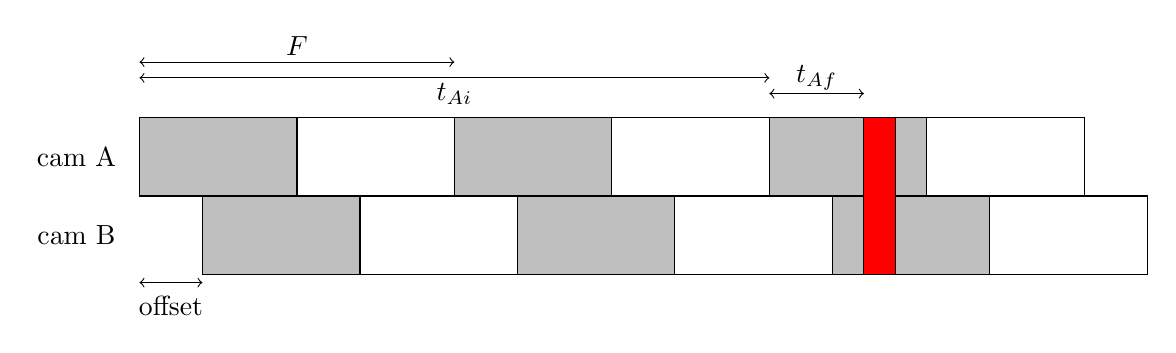
\begin{tikzpicture}[scale=1.0]
	\def\blkw{4}
	\def\blkh{1}

	\newcommand*{\mybox}[1]{%
	\draw (#1) rectangle +(\blkw,\blkh);
	\draw [fill=gray!50] (#1) rectangle +(0.5*\blkw,\blkh);
	}

	\mybox{0,0}
	\mybox{\blkw,0}
	\mybox{2*\blkw,0}

	\node at (-0.2*\blkw,0.5*\blkh) {cam A};
	\node at (-0.2*\blkw,-0.5*\blkh) {cam B};

	\mybox{0.2*\blkw,-\blkh}
	\mybox{1.2*\blkw,-\blkh}
	\mybox{2.2*\blkw,-\blkh}

	\draw [fill=red] (2.3*\blkw,\blkh) rectangle +(0.1*\blkw,-2*\blkh);
	\draw [<->] (0,1.7*\blkh) -- +(1.0*\blkw,0);
	\draw [<->] (0,1.5*\blkh) -- +(2.0*\blkw,0);
	\draw [<->] (2*\blkw,1.3*\blkh) -- +(0.3*\blkw,0);

	\node at (0.5*\blkw,1.9*\blkh) {$F$};
	\node at (1.0*\blkw,1.3*\blkh) {$t_{Ai}$};
	\node at (2.15*\blkw,1.5*\blkh) {$t_{Af}$};

	\draw [<->] (0,-1.1*\blkh) -- +(0.2*\blkw,0);
	\node at (0.1*\blkw,-1.4*\blkh) {offset};
\end{tikzpicture}
\end{document}

